\documentclass{report}

% Packages for math symbols and equations
\usepackage[T1]{fontenc}
\usepackage[utf8]{inputenc}

\usepackage[margin=1.4in]{geometry}
\usepackage{graphicx}

\usepackage{amssymb,amsthm, amsmath}
%\usepackage{mathtools}
%\numberwithin{equation}{section}

\usepackage[
natbib,
style=alphabetic,
maxbibnames=10,  
sorting=ydnt,
url=false,
doi=false,
sortcites,
defernumbers,
backref,
backend=biber
]{biblatex}
\addbibresource{bibliography.bib}

\usepackage{hyperref}

\usepackage{todonotes}
%\setuptodonotes{inline}
\usepackage{url}

\usepackage[nameinlink, capitalise, noabbrev]{cleveref}

\usepackage{xfrac}
\usepackage{nicefrac}

\usepackage{soul}

\usepackage{bbm}

\usepackage{enumitem}

%For double brackets \llbracket \rrbracket
\usepackage{stmaryrd}

\crefname{assumption}{Assumption}{Assumptions}

\newtheorem{theorem}{Theorem}

\newtheorem{proposition}{Proposition}[section]
\newtheorem{lemma}{Lemma}[section]
\newtheorem{corollary}{Corollary}[section]
\theoremstyle{remark}
\newtheorem{remark}{Remark}[section]


\theoremstyle{definition}
\newtheorem{example}{Example}[section]
\newtheorem{counterexample}{Counterexample}[section]
\newtheorem{definition}{Definition}[section]
\newtheorem{assumption}{Assumption}

%\numberwithin{equation}{section}

%\renewcommand{\baselinestretch}{2}

%\newcounter{hypcounter}

\newcommand{\N}{\mathbb{N}}
\newcommand{\Z}{\mathbb{Z}}
\newcommand{\R}{\mathbb{R}}
%\DeclareMathOperator{\dom}{dom}
\newcommand{\closure}[1]{\overline{#1}}
\newcommand{\norm}[1]{\left\Vert #1 \right\Vert}
\newcommand{\seminorm}[1]{\left[ #1 \right]}
\newcommand{\abs}[1]{\left\vert #1 \right\vert}
%\DeclareMathOperator{\divtmp}{div}
\renewcommand{\div}{\divtmp}
% \DeclareMathOperator{\argmin}{arg\,min}
% \DeclareMathOperator{\argmax}{arg\,max}
% \DeclareMathOperator{\esssup}{ess\,sup}
% \DeclareMathOperator{\essinf}{ess\,inf}
\renewcommand{\st}{\,:\,}
% \DeclareMathOperator{\supp}{supp}
\newcommand{\dx}{\,\mathrm{d}x}
\renewcommand{\d}{\,\mathrm{d}}
\newcommand{\dH}{\,\mathrm{d}\mathcal{H}^{n-1}(x)}
% \DeclareMathOperator{\sign}{sign}
\newcommand{\eps}{\varepsilon}
% \DeclareMathOperator{\dist}{dist}
% \DeclareMathOperator{\Lip}{Lip}
\newcommand{\KR}{\mathrm{KR}}
\newcommand{\C}{\mathrm{C}}
\renewcommand{\L}{\mathrm{L}}
\newcommand{\W}{\mathrm{W}}
\newcommand{\M}{\mathcal M}
\newcommand{\grad}{\nabla}
\newcommand{\hess}{\mathrm{D}^2}
\newcommand{\defeq}{:=}
% \DeclareMathOperator{\diam}{diam}
\newcommand{\Set}[1]{\left\lbrace#1\right\rbrace}
\newcommand{\scale}{\eps}
\newcommand{\res}{\delta}


\newcommand{\wto}{\rightharpoonup}
\newcommand{\wsto}{\overset{\ast}{\rightharpoonup}}
\newcommand{\strictto}{\overset{\mathrm{str}}{\rightharpoonup}}

\newcommand{\rev}{\color{magenta}}
\renewcommand{\rev}{}
\newcommand{\red}{\color{red}}
\newcommand{\blue}{\color{blue}}
\newcommand{\nc}{\normalcolor}


% Lie math operators
\DeclareMathOperator{\toledo}{T}
\DeclareMathOperator{\isom}{Isom}
\DeclareMathOperator{\bus}{b}
\DeclareMathOperator{\ii}{i}
\DeclareMathOperator{\spa}{span}
\DeclareMathOperator{\class}{C}
\DeclareMathOperator{\diam}{diam}
\DeclareMathOperator{\diag}{diag}
\DeclareMathOperator{\U}{{\mathrm{U}}}
\DeclareMathOperator{\SL}{{\mathrm{SL}}}
\DeclareMathOperator{\SU}{{\mathrm{SU}}}
\DeclareMathOperator{\su}{{\mathfrak{su}}}
\DeclareMathOperator{\PSL}{{\mathrm{PSL}}}
\DeclareMathOperator{\GL}{{\mathrm{GL}}}
\DeclareMathOperator{\SO}{{\mathrm{SO}}}
\DeclareMathOperator{\PGL}{{\mathrm{PGL}}}
\DeclareMathOperator{\PO}{{\mathrm{PO}}}
\DeclareMathOperator{\PSO}{{\mathrm{PSO}}}
\DeclareMathOperator{\id}{id}
\DeclareMathOperator{\inte}{int}
\DeclareMathOperator{\LC}{LC{}}
\DeclareMathOperator{\F}{Frenet{}}
\DeclareMathOperator{\lie}{Lie}
\DeclareMathOperator{\Ker}{Ker}
\DeclareMathOperator{\ad}{ad}
\DeclareMathOperator{\Hff}{dim_{Hf{}f}}
\DeclareMathOperator{\vol}{Vol}
\DeclareMathOperator{\rk}{rank}
%\DeclareMathOperator{\jac}{jac}
\DeclareMathOperator{\gap}{{\sf{gap}}}
\DeclareMathOperator{\ann}{Ann}
\DeclareMathOperator{\Ad}{Ad}

\newcommand{\restr}{\mathbin{\vrule height 1.6ex depth 0pt width
0.13ex\vrule height 0.13ex depth 0pt width 1.3ex}}

% Title page information
\title{Limit sets of Anosov representations}
\author{Giorgos}
\date{\today}

\begin{document}

\maketitle

\tableofcontents

\chapter{Introduction}
\section{Lie group preliminaries}
We fix the Cartan subalgebra $\mathfrak a$ of $\SL(d,\mathbb R)$:
\[
    \mathfrak a = \left\{
        \diag(\alpha_1, \ldots, \alpha_d) : \alpha_1 + \cdots \alpha_d = 0
    \right\}
\]
and the Weyl chamber $\mathfrak a^+$ of $\SL(d,\mathbb R)$
\[
    \mathfrak a^+ = \left\{
        \diag(\alpha_1, \ldots, \alpha_d) : \alpha_1 \geq \cdots \geq \alpha_d
    \right\}.
\]
Denoting with $K = \SO(d, \mathbb R), A^+ = e^{\mathfrak a^+} $, we have the Cartan decomposition:
\begin{align*}
    \mathfrak{sl}(d, \mathbb R) &\rightarrow K \times A^+ \times K\\
    g &\mapsto (k_g, a_g, l_g) 
\end{align*}
such that $g = k_g a_g l_g$.
In particular $a_g = \diag(\sigma_1(g), \ldots, \sigma_d(g))$ with $\sigma_1 \geq \cdots \geq \sigma_d(g)$,
where $\sigma_i(g)$ is the $i$-th singular value of $g$, i.e.\ eigenvalue of $g^t \cdot g$.

We will use the spaces
\[
    U_p(g) = \mathbb R u_1(g) \oplus \cdots \oplus \mathbb R u_p(g)   
\]
where $u_i(g) = k_g \cdot e_i$.
One can easily show that the decomposition
\[
    g^{-1} \cdot U_p(g) \oplus U_{d-p}(g^{-1})
\]
is orthogonal with respect to the standard inner product and that
$u_p(g^{-1}) = l_g^{-1} e_{d-p+1}(g).$
\section{Limit set preliminaries}
\begin{definition}
For $p \in \{2, \ldots, d\}, s\in \mathbb R $
and $g \in SL(d, \mathbb R)$ 
we denote with $\tilde \Psi_s^p(g), \Psi_s^p(g): \SL(d, \mathbb R) \to \mathbb R$ the functional:
\begin{align*}
\Psi_s^p(g) &= 
    \alpha_{12}(a(g)) + \cdots + \alpha_{1(p-1)}(a(g)) + (s - (p-2))\alpha_{1p}(a(g))\\
\tilde \Psi_s^p(g) &= 
    \left( \frac{\sigma_2}{\sigma_1}\cdots\frac{\sigma_{p-1}}{\sigma_1}(g)\right) 
    \left( \frac{\sigma_{p-1}}{\sigma_1}(g) \right)^{s - (p-2)}
\end{align*}
\end{definition}
\begin{remark}
    We have $\alpha_{ij}(a) = a_i - a_j, a_i(g) = \log (\sigma_i(g))$ and 
    \[
        \Psi_s^p(g) = \log \tilde \Psi_s^p(g)
    \]
and that
\begin{align*}
    \min_{p \in \llbracket 2, d \rrbracket} 
    \left\{ 
        \sum_{|\gamma| = T} 
            \frac{\sigma_2}{\sigma_1}\cdots\frac{\sigma_{p-1}}{\sigma_1}(g) 
            \left( \frac{\sigma_{p-1}}{\sigma_1}(g) \right)^{s - (p-2)}
    \right\} = 
    \sum_{|\gamma| = T} e^{-\max\limits_{p \in \llbracket 2, d \rrbracket} \Psi_s^p(g)}
\end{align*}
\end{remark}

\begin{remark}
For any $g \in \SL(d, \mathbb R)$ we have that:
\[
    \max_{p \in \llbracket 2, d \rrbracket} \Psi_s^p(g) = \Psi_s^{p_0}(g) \text{ for } s \in [p_0 - 2, p_0 -1].
\]
Indeed, a quick calculation shows that for $s \geq 0$ and $p \in \llbracket 2, d \rrbracket$:
\[
    \Psi_s^p(g) \leq \Psi_s^p(g) \text{ if and only if } s \geq p-1.
\]
and that equality holds in the case $s = p - 1$.
Thus for $s \in [p - 2, p-1]$ we have that
\begin{align*}
    s \geq p-2, \ldots, 1 &\text{ implies that } \Psi_s^p(g) \geq \ldots \geq \Psi_s^{2}(g)\\
    s \leq p, \ldots, d-1 &\text{ implies that } \Psi_s^p(g) \leq \ldots \leq \Psi_s^d(g)
\end{align*}
Another way to see this (refer to \cref{fig:max}) is to note that $\Psi_s^2(g), \cdots, \Psi_s^d(g)$ is a sequence of functions that are affine in $s$, with slopes $\alpha_{12}(g) \leq \cdots \leq \alpha_{1d}(g)$ and that they satisfy $\Psi_1^2(g) = \Psi_2^2(g), \Psi_2^3(g) = \Psi_3^4(g) \ldots, \Psi_{d-2}^{d-1}(g) = \Psi_{d-2}^d(g)$.
\begin{figure}[h]
    \centering
    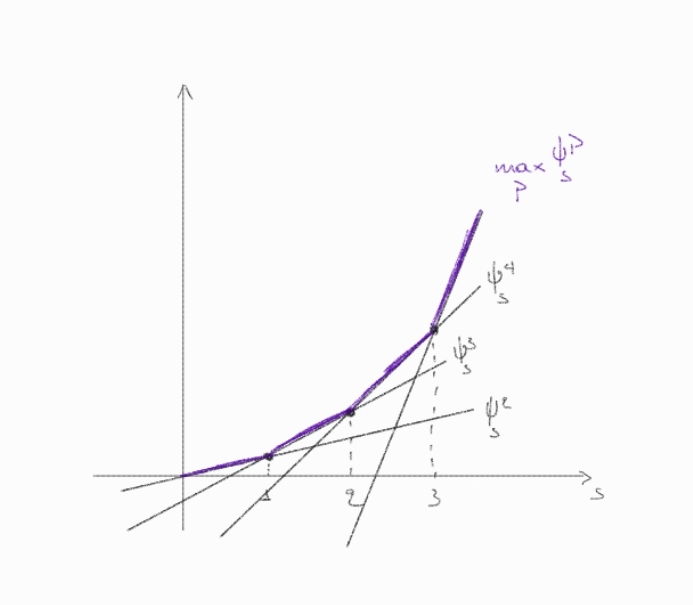
\includegraphics[width=0.4\textwidth]{max.jpg}
    \caption{Visual illustration that $\max_p\Psi_s^p(g) = \Psi_s^{p_0}(g) \text{ for } s \in [p_0 - 2, p_0 -1]$.}
    \label{fig:max}
\end{figure}    
\end{remark}


The following definition comes from \cite{ledrappier_dimension_2023}, in the special case of projective Anosov representations ($P = {1}$):
\begin{definition}
    For $s \geq 0$ we consider the Falconer functional $F_s : \SL(d, \mathbb R) \to \mathbb R$ by:
    \[
        F_s(g) = \min 
        \left\{
            \sum_{j=2}^d s_j \alpha_{1j}(a(g)) : s_j \in (0,1], \sum_{j=2}^d s_j = s 
        \right\},
    \]
    and define the Falconer dimension $\dim_F(\rho)$ of $\rho$ to be its critical exponent:
    \[
        \dim_F(\rho) = \inf
        \left\{
            s > 0: \sum_{\gamma \in \Gamma} e^{-F_s(\rho(\gamma))} < \infty
        \right\}.
    \]
\end{definition}

\begin{remark}
    Using elementary computations one may prove that for all $s \geq 0$:
    \[
        F_s(g) = \max_{p \in \llbracket 2, d \rrbracket} \Psi_s^p(g)
    \]
\end{remark}

\begin{definition}
Let $\rho: \Gamma \to \SL(d, \mathbb R)$ be a linear representation and $p \in \llbracket 1, d-1 \rrbracket$.
We say that $\rho$ is $p$-Anosov if there exist constants $\mu, C>0$ such that for all $\gamma \in \Gamma$:
\[
    \frac{\sigma_{p+1}}{\sigma_p}(\rho(\gamma)) \leq C e^{-\mu |\gamma|}.
\]
One can show that in that case there exist equivariant continuous maps $\xi^p: \hat \Gamma \to \mathcal G_p(\mathbb R^d) , \xi^{d-p}: \hat \Gamma \to \mathcal G_{d-p}(\mathbb R^d)$ that are transverse and restrict to
\[
    \xi^p(\gamma) = U_p(\rho(\gamma)), \xi^{d-p}(\gamma) = U_{d-p}(\rho(\gamma))
\]
for $\gamma \in \Gamma$, where $U_p(\gamma), U_{d-p}(\gamma)$ denote the flags 
\todo{Figure out what this exactly means}
corresponding to  $\rho(\gamma)$.
\end{definition}
\chapter{Upper bound}
\section{Proof of bound}
\begin{lemma}[Upper bound for dimension]\label{lem:upper_bound}
Let $\rho: \Gamma \to \SL(d, \mathbb R)$ be a projective Anosov representation. 
Then:
\[
    \dim_H(\xi^1 (\partial \Gamma) ) \leq \dim_F(\rho).
\]
\end{lemma}
\begin{remark}
    The idea of the proof of \cref{lem:upper_bound} is to find a covering whose Hausdorff content is dominated by the Dirichlet series of some functional $\Psi_s^p$, which will in turn imply that $\dim_H(\xi^1(\partial \Gamma)) \leq h_\rho(\Psi^p) $.
    Choosing then the most "effective" cover (i.e.\ the one which yields the smallest Hausdorff content up to a constant) we obtain that
    \[
        \dim_H(\xi^1(\partial \Gamma)) \leq h_\rho(\max_p \Psi^p)
    \]
    To obtain this we first cover $\xi^1(\partial \Gamma)$ by the bassins of attraction $\rho(\gamma) \cdot B_{\alpha_1, \alpha} (\rho(\gamma))$ for $\gamma \in \Gamma$ satisfying $|\gamma| = T$.
    Then we cover each bassin by an ellipsoid of axes lengths
    \[
        \frac{1}{\sin(\alpha)} \frac{\sigma_2}{\sigma_1}(\rho(\gamma)), \ldots, 
        \frac{1}{\sin(\alpha)} \frac{\sigma_d}{\sigma_1}(\rho(\gamma)).
    \]
    Finally we cover each ellipsoid by balls of some fixed radius $r>0$.
    It can be shown by comparing the series appearing in the Hausdorff content of each resulting cover that the most "effective" choice of $r$ depends only on the Hausdorff exponent $s > 0$ and in any case will be to have $r$ equal (up to a constant) to the the length of an axis of the ellipsoid, i.e.\
    \[
        r \in \left\{
            \frac{1}{\sin(\alpha)} \frac{\sigma_2}{\sigma_1}(\rho(\gamma)), \ldots, 
            \frac{1}{\sin(\alpha)} \frac{\sigma_d}{\sigma_1}(\rho(\gamma)).    
        \right\}
    \]
    In particular, when $s \in [p-2, p-1]$, the most effective choice is $r = \sigma_p(\rho(\gamma))/\sigma_1(\rho(\gamma))$, whose Hausdorff content is dominated by the Dirichlet series of $\Psi_s^p$.
\end{remark}

\begin{proof}[Proof of \cref{lem:upper_bound}]
Let $p \in \llbracket 2, d \rrbracket$.
Then using \cref{prop:basin_covering}, \cref{lem:boundary_covering}, and \cref{lem:ellipsoid_covering} we have that for $T>0$ large enough, $\xi^1(\partial \Gamma)$ is covered by the family
\[
    \mathcal U_T = \left\{ \rho(\gamma) B_{\alpha_1, \alpha}(\rho(\gamma)) : |\gamma| = T \right\},
\]
and that each basin $\rho(\gamma) B_{\alpha_1, \alpha}(\rho(\gamma))$ is in turn covered by
\[
    2^{p-2} \cdot \frac{\sigma_p(g)^{p-2}}{\sigma_2(g) \cdots \sigma_{p-1}(g)}
\]
many balls of radius
\[
    \sqrt{d-1} \frac{1}{\sin \alpha} \frac{\sigma_p(g)}{\sigma_1(g)}.
\]
By the definition of the Hausdorff measure, for $s \geq 0$:
\begin{align*}
    \mathcal H^s(\xi^1(\partial \Gamma)) &\leq
    \sum_{|\gamma| = T}
        2^{2p+1} \cdot 
        \frac{\sigma_2(\rho(\gamma))}{\sigma_1(\rho(\gamma))} \cdots 
            \frac{\sigma_{p-1}(\rho(\gamma))}{\sigma_1(\rho(\gamma))}
        \left(
            \frac{\sigma_p(\rho(\gamma))}{\sigma_1(\rho(\gamma))}
        \right)^{-(p-2)}
        \left(
            \sqrt{d-1} \frac{1}{\sin \alpha} \frac{\sigma_p(\rho(\gamma))}{\sigma_1(\rho(\gamma))}
        \right)^s =\\
        &=
        2^{2p+1} \cdot \left( \frac{\sqrt{d-1}}{\sin \alpha}\right)^s  
        \sum_{|\gamma| = T} 
        \frac{\sigma_2(\rho(\gamma))}{\sigma_1(\rho(\gamma))} \cdots 
            \frac{\sigma_{p-1}(\rho(\gamma))}{\sigma_1(\rho(\gamma))}
        \left(
            \frac{\sigma_p(\rho(\gamma))}{\sigma_1(\rho(\gamma))}
        \right)^{s-(p-2)} =\\
        &=
        2^{2p+1} \cdot \left( \frac{\sqrt{d-1}}{\sin \alpha}\right)^s  
        \sum_{|\gamma| = T}
        e^{-\left( \alpha_{1 2} + \ldots + \alpha_{1 (p-1)} + (s - (p-2))\alpha_{1 p} \right)\rho(\gamma)}\\
        &=
        2^{2p+1} \cdot \left( \frac{\sqrt{d-1}}{\sin \alpha}\right)^s  
        \sum_{|\gamma| = T}
        e^{-\Psi_s^p(\rho(\gamma))}
\end{align*}
and thus
\begin{align*}
    \mathcal H^s(\xi^1(\partial \Gamma)) \leq
    2^{2p+1} \cdot \left( \frac{\sqrt{d-1}}{\sin \alpha}\right)^s
    \sum_{|\gamma| = T}
    e^{-\max_p \Psi_s^p(\rho(\gamma)) }\lesssim \sum_{|\gamma| = T} e^{-F_s(\rho(\gamma))}.
\end{align*}
To see that the above implies the upper bound, consider some $s > \dim_F(\rho)$.
By the definition of the Falconer dimension, this implies that the Dirichlet series corresponding to the Falconer functional converges:
\[
    \sum_{\gamma \in \Gamma} e^{-F_s(\rho(\gamma))} < \infty
\]
and in particular
\[
    \mathcal H^s(\xi^1(\partial \Gamma)) \leq 
    \lim_{T \to \infty} e^{-F_s(\rho(\gamma))} = 0.
\]
\end{proof}

\section{Lemmata}
\begin{definition}
    Let $V$ be a finite-dimensional $\mathbb R$-vector space.
    We consider a decomposition
    \[
        V = \mathbb R u_1 \bigoplus \cdots \bigoplus \mathbb R u_d
    \] 
    be a direct decomposition that is orthogonal with respect to a fixed inner-product over $V$.
    Given $\beta_2 \geq \ldots \beta_d > 0$, we define an ellipsoid with axes $u_1 \oplus u_p(g)$ and lengths $\beta_p$ to be the image of
    \[
        \left\{
            v = \sum_1^d v_i u_i\in V : \sum_2^d \left( \frac{v_j}{\beta_j} \right)^2 \leq 1
        \right\}
    \]
    through the projection $ V \to \mathbb P (V)$.
\end{definition}
\begin{figure}[h]
    \centering
    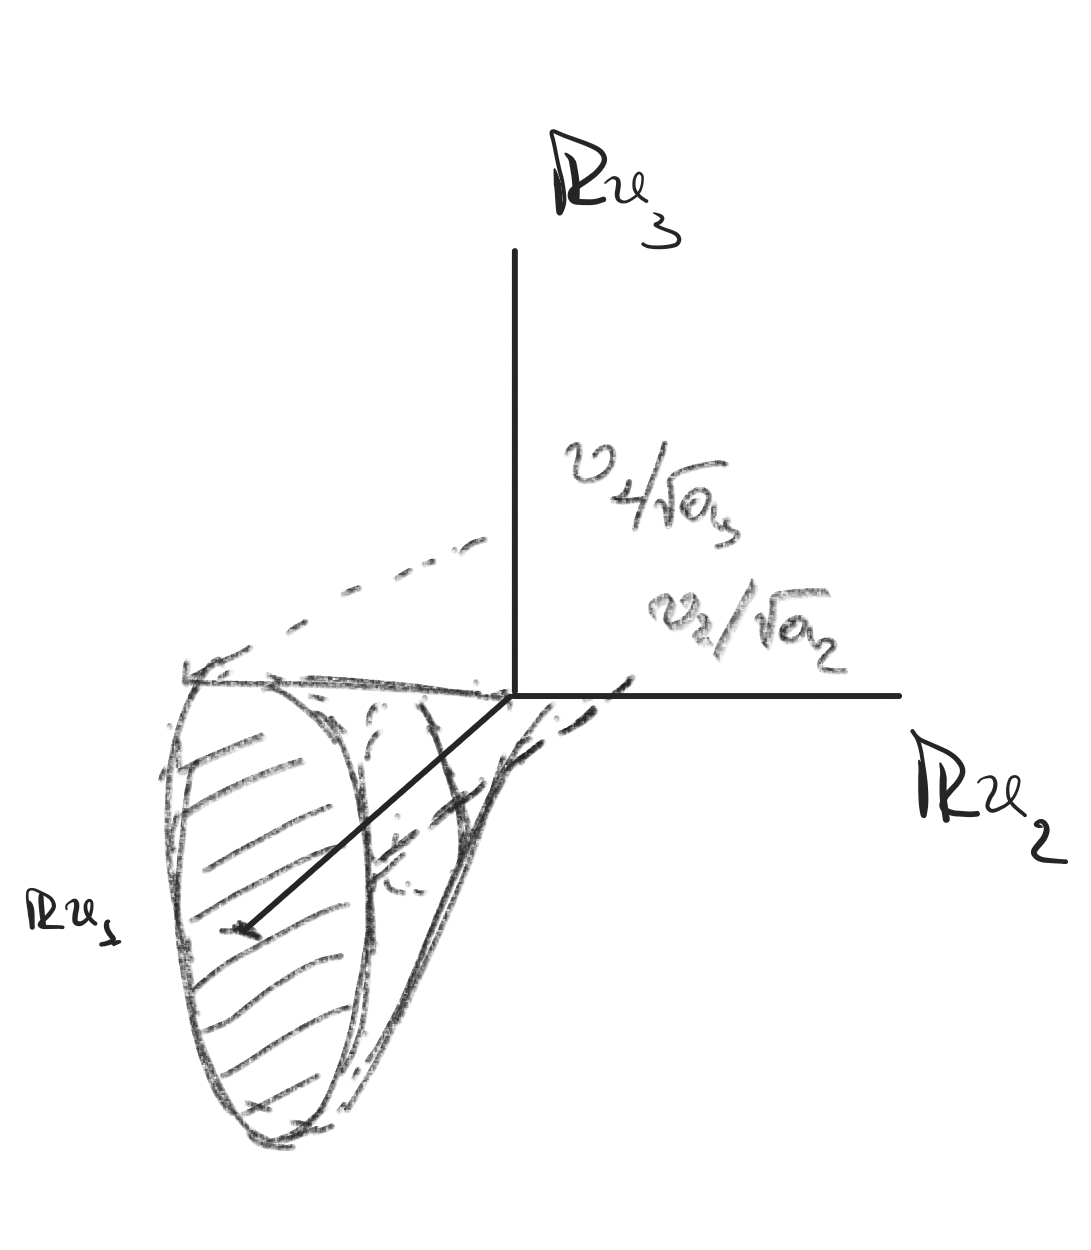
\includegraphics[width=0.4\textwidth]{ellipsoid.jpg}
    \caption{Depiction in $\mathbb R^3$ of an ellipsoid of $\mathbb P(\mathbb R^2)$}
    \label{fig:ellipsoid}
\end{figure}    

The following aims to be something along the lines of \cite*[Lemma 2.4]{pozzetti_anosov_2023}:
\begin{lemma}\label{lem:angle}
    Let $\rho: \Gamma \to \SL(d, \mathbb R)$ be a projective Anosov representation.
    For $\alpha > 0$ small enough, there exists $L>0$ such that for any geodesic ray $(a_j)_j$ through $e$ we have:
    \[
        \angle(U_1(\rho(a_i)), U_{d-1}(\rho(a_0))) > \alpha
    \]
    when $|a_i|, |a_0| > T$.
\end{lemma}
\begin{proof}
Assume the contrary for the shake of contradiction.
Then (see Figure \ref{fig:angle} ) for each $n>0$ there exists a geodesic ray  $a^n$ through $e$ such that 
\[
    |a_n^n|, |a_0^n| > n \text{ and }
    \angle(U_1(\rho(a_n^n)), U_1(\rho(a_0^n))) < \frac{1}{n}.
\]
Due to compactness of $\partial \Gamma$ we may assume (up to a subsequence) that
$a^n \to x$ in $\partial \Gamma$ for some $x \in \partial \Gamma$.
Then 
\todo{Not sure if this is true.}
$a^n_n, a_0^n \to x$ in $\hat \Gamma$ which implies
\[
    \angle (\xi^1(x), \xi^{d-1}(x)) = 0
\]
using the fact that the limit maps $\xi^1, \xi^{d-1}$ are continuous, which contradicts their tranversality.
\end{proof}
\begin{figure}[h]
    \centering
    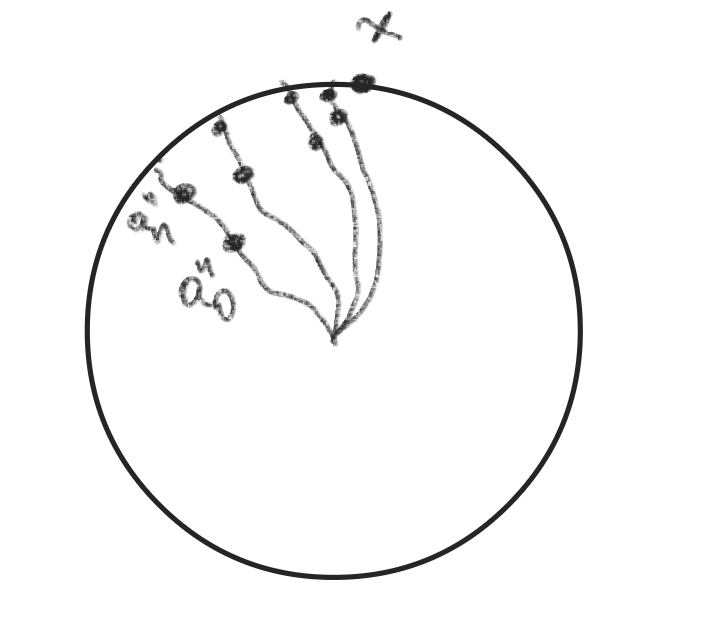
\includegraphics[width=0.3\textwidth]{angle.jpg}
    \caption{Situation in \cref{lem:angle}}
    \label{fig:angle}
\end{figure}    

The following is \cite[Proposition 3.5]{pozzetti_anosov_2023}.
\begin{lemma}\label{lem:boundary_covering}
Let $\rho: \Gamma \to SL(d, \mathbb R)$ be projective Anosov.
Then for $\alpha > 0$ small enough, there exists some $T_0 > 0$ such that for all $T \geq T_0$ the family
\[
    \mathcal U_T = \left\{ \rho(\gamma) B_{\alpha_1, \alpha}(\rho(\gamma)) : |\gamma| = T \right\}
\]
is an open covering of $\xi^1(\partial \Gamma)$.
\end{lemma}
\begin{proof}
    Let $\alpha, T > 0$ be as in the statement of \cref{lem:angle} and $x \in \partial \Gamma$ be represented by a geodesic ray $(\gamma_j)_{j\geq 0}$ starting from $e$.
    Then $(\gamma_T^{-1} \gamma_j)_j$ is a geodesic ray starting from $(\gamma_T)^{-1}$ that passes through $e$, so
    \[
        \angle (U_1(\rho(\gamma_T^{-1}\gamma_j)), U_{d-1}(\rho(\gamma_T^{-1}))) > \alpha
    \]
    as implied by \cref{lem:angle}.
    Taking the limit $j \to \infty$ and using the equivariance of the limit map, we obtain
    \[
        \angle (\rho(\gamma_T^{-1})\xi^1(x), U_{d-1}(\rho(\gamma_T^{-1}))) > \alpha
    \]
    and thus $\xi^1(x) \in \rho(\gamma_T) \cdot B_{\alpha_1, \alpha}(\rho(\gamma_T))$.
\end{proof}

The following is \cite[Proposition 3.8]{pozzetti_anosov_2023}.
\begin{proposition}\label{prop:basin_covering}
For each $g\in \SL(d, \mathbb R), \alpha > 0$, 
the basin of attraction $g \cdot B_{\alpha_1, \alpha}(g)$ lies in the ellipsoid with axes $u_1(g) \oplus u_p(g)$ with lengths
\[
    \frac{1}{\sin \alpha} \cdot \frac{\sigma_p(g)}{\sigma_1(g)}
\]
\end{proposition}
\begin{proof}
Using the definition of the basin of attraction (see \cref{fig:projection} ), we have that $w = w_1 u_1(g^{-1}) + \cdots + w_d u_d(g^{-1}) \in B_{\alpha_1, \alpha}(g)$ if and only if
\[
    w_d^2 \geq (\sin \alpha)^2 \sum_1^d w_i^2.
\]
Considering now some $v = v_1 u_1(g) + \cdots + v_d u_d(g) \in g \cdot B_{\alpha_1, \alpha}(g)$
we have that
\begin{align*}
    w = g^{-1} v &= v_1 \sigma_1(g)^{-1} l_g^{-1} e_1(g) + \cdots v_d \sigma_d(g)^{-1} l_g^{-1} e_d(g)\\
    &= v_1 \sigma_1(g)^{-1} u_{d}(g^{-1}) + \cdots v_d \sigma_d(g)^{-1} u_1(g^{-1})
\end{align*}
where we used that $u_p(g^{-1}) = l_g^{-1} e_{d+1-p}$.
Hence
\[
    \sigma_1(g)^{-2} \cdot v_1^2 \geq (\sin a)^2 \sum_1^d \sigma_i(g)^{-2} v_i^2.
\]
\end{proof}
\begin{figure}[h]
    \centering
    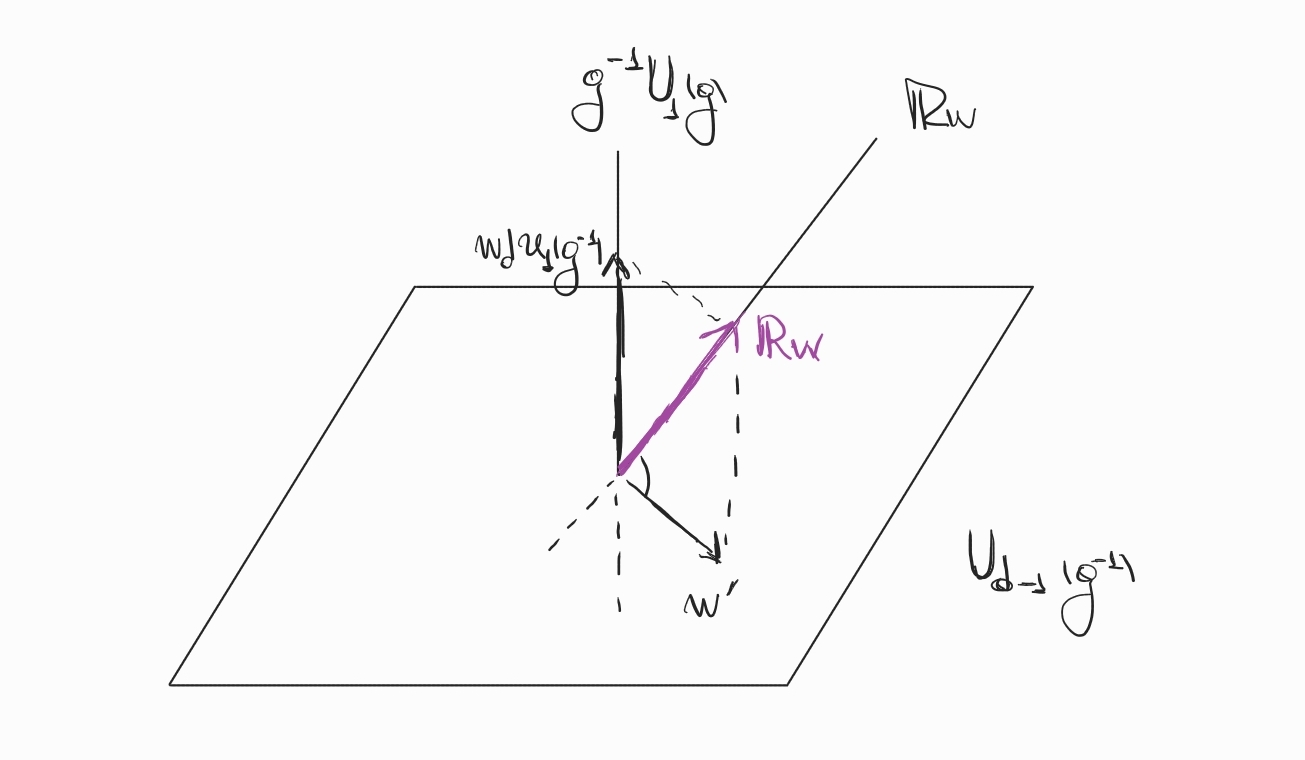
\includegraphics[width=0.4\textwidth]{projection.jpg}
    \caption{Aid for \cref{prop:basin_covering}}
    \label{fig:projection}
\end{figure}

The following is \cite[Lemma 3.7]{pozzetti_anosov_2023}:
\begin{lemma}\label{lem:ellipsoid_covering}
For any $p \in \llbracket 2, d \rrbracket$, an ellipsoid in $\mathbb P(\mathbb R^d)$ of axes lengths $\beta_2, \cdots, \beta_d$ is covered by
\[
    2^{p - 2} \frac{\beta_2 \cdots \beta_{p-1}}{\beta_p^{p-2}}
\]
many (projected) balls of radius $\sqrt{d-1} \beta_p$.
\end{lemma}
\begin{proof}
We assume that $E$ is an ellipsoid about $\mathbb R e_1$, so it suffice to cover its intersection $E_1 = E \cap U_1 \subseteq \mathbb R^{d-1}$ with the affine chart $U_1 = \{ [x_1: \ldots, x_d ] \in \mathbb P(\mathbb R^d) : x_1 \neq 0 \}$.
Clearly $E_1 \subseteq [-\beta_2, \beta_2] \times \ldots \times [-\beta_d, \beta_d]$, so we proceed by covering the rectangle with side-lengths $2\beta_2, \ldots, 2\beta_d$.
Clearly each interval $(-\beta_j, \beta_j)$ is contained in the union of $\lceil \beta_j/\beta_p \rceil$ intervals of length $2\beta_p$, thus $E_1$ is contained in the union of
\[
    \left\lceil \frac{\beta_2}{\beta_p} \right\rceil \cdots \left\lceil \frac{\beta_{p-1}}{\beta_p} \right\rceil =
    \left\lceil \frac{\beta_2}{\beta_p} \right\rceil \cdots \left\lceil \frac{\beta_d}{\beta_p} \right\rceil
\]
many squares of side-length $2\beta_p$.
Since each such product is contained in a $(d-1)$-ball of radius $\sqrt{d-1} \beta_p$ we may use at most
\[
    \left\lceil \frac{\beta_2}{\beta_p} \right\rceil \cdots \left\lceil \frac{\beta_{p-1}}{\beta_p} \right\rceil \leq
    \sum_{i \in \{ 0,1 \}^{p-2} } \prod_{j = 2}^{p-1} \left( \frac{\beta_j}{\beta_p} \right)^{i_j} \leq 2^{p-2} \frac{\beta_2}{\beta_p} \cdots \frac{\beta_{p-1}}{\beta_p}
\]
many $(d-1)$-balls of radius $\sqrt{d-1}\beta_p$ to cover $E_1$.
\end{proof}

The following can be found in \cite[Proposition 3.3]{pozzetti_anosov_2023}:
\begin{proposition}
    Let $\rho: \Gamma \to SL(d, \mathbb R)$ be projective Anosov and $\alpha > 0$
    Then there exist $c_0, c_1 > 0$ that depends only on $\alpha$ and $\rho$ such that for all $\gamma \in \Gamma$:
    \[
        (\xi^1)^{-1}(B_{\alpha_1, \alpha}(\rho(\gamma))) \subseteq C_{c_0,c_1}^\infty(\gamma)
    \]
\end{proposition}
\begin{proof}
    We begin by noting that it suffices to show this for all but finitely many $\gamma \in \Gamma$, since then we may alter the constants to satisfy the wanted inclusion also for the finitely many remaining $\gamma \in \Gamma$. Given this, we shall assume that $|\gamma| \geq l_0$ where $l_0 > 0$ is such that $Ce^{-\mu l_0} < 1$ and $C, \mu > 0$ are the constants appearing in the definition of the Anosov property of $\rho$..

    Suppose $x \in \partial \Gamma$ such that $\xi^1(x) \in B_{\alpha_1, \alpha}(\rho(\gamma))$, and consider a geodesic ray $a_j \to x$ starting from $a_0 = e$.
    To prove the result, it suffices to find constants $c_0, c_1$ independent of $\gamma$ and a ($c_0$, $c_1$)-quasi-geodesic from $\gamma^{-1}$ to $x$ that passes through $e$ and stays at a bounded distance from $(a_j)_{j=0}^\infty$

    Using \cite[Proposition 2.5]{pozzetti_anosov_2023} we have that
    $d(\xi^1(a_j), U_{d-1}(\rho(\gamma^{-1}))) \leq C e^{-\mu j}$, 
    so there exists some $L>0$ that depends only on $\alpha$ 
    such that for all $j\geq L: U_1(\rho(a_j))\in B_{\alpha_1, \alpha}(\rho(\gamma))$ and in particular
    \[
        d(\xi^1(a_j), \gamma^{-1}) = d(U_1(\rho(a_j)), U_1(\rho(\gamma^{-1}))) \geq 
        d(U_1(\rho(a_j)), U_{d-1}(\rho(\gamma^{-1}))) > \sin\alpha.
    \]
    Along with the uniform continuity of $\xi^1: \Gamma \cup \partial \Gamma \to \mathbb P(\mathbb R^d)$ this implies there exists some $\alpha' > 0$ and $L>0$ such that for all $j\geq L$:
    \[
        d(a_j, \gamma^{-1}) \geq \alpha'.
    \]
    Upon considering a large $L$, we may also assume that $|a_L| = L > l_0$. Note that both $\alpha'$ and $L$ do not depend on each $\gamma$ but only on $\rho$ and $\alpha$.

    Using some geometric group theory, we can show that for all $j \geq L$
    \[
        d(\gamma^{-1}, a_j) > \alpha' \Rightarrow
        d([\gamma^{-1}, a_j], e) < \alpha''
    \]
    for some $\alpha''$ that depends only on $\Gamma$ and $\alpha'$, where $[a_j, \gamma^{-1}]$ denotes the geodesic segment connecting $\gamma^{-1}$ and $a_j$.

    Consider the concatenation $(a_j')_{j=L-K}^\infty$ of $[\gamma^{-1},a_L]$ and $[a_L, x]$.
    To find quasi-geodesic-constants that are uniform in $\gamma$, we note that for any $c_0 \geq 1, c_1 \geq 0$:
    \[
        c_0^{-1} |i - j| - c_1 \leq d(a_i', a_j') = d(a_i, a_j) \leq d(a_i) c_0^ |i - j| + c_1 
        \text{ when } i,j \geq L \text{ or } i,j \leq L
    \]
    and that the upper bound follows trivially by the triangle inequality. 
    
    For the lower bound we proceed in two steps. 
    First we bound the distance of $\gamma^-1 = a_{L-K}'$ to $a_{L+j}$ for $j\geq 0$:
    \begin{align*}
        d(a_{L-K}', a_{L+j}') 
        &\geq \nu (|a_{L+j}| - |\gamma^{-1}|) - c_0' -c_1'|\log(d(U_1(\rho(a_{L+j})), U_1(\rho(\gamma^{-1}))))| \geq\\
        &\geq \nu((L+j) + (K-L)) - c_0' -c_1'|\log(\sin a)| \geq\\
        &= c_0^{-1} (j+K) - c_1
    \end{align*}
    for $c_0 = \nu^{-1}, c_1 = c_0' + c_1'|\log(\sin \alpha)|$.
    The first inequality comes from \cite[Lemma 3.9]{pozzetti_anosov_2023}. For the second inequality we estimate $|\gamma^{-1}|$ from below using the triangle inequality.
    We are now ready to show that the concatenation $(a_j')_j$ is indeed a ($c_0$, $c_1$)-geodesic:
    \begin{align*}
        d(a_{L+j}, a_{L-i}) &\geq d(a_{L+j},a_{L_K}) - d(a_{L_K}, a_{L-i}) \geq
        c_0^{-1} (j+K) - c_1 - (K - i) \geq\\
        &\geq c_0^{-1} (j+i) - c_1.
    \end{align*}

    Note however that $(a_j')$ does not necessarily lie in $C_\infty^{c_0, c_1}$ since it may not pass through $e$.
    For this reason we some $L - K \leq i_0\leq L$ such that $|a_{i_0}| < \alpha''$, the existence of which is guaranteed by the fact that $d([\gamma^{-1}, a_L], \epsilon) < \alpha''$.
    We then consider alter $(a_j')$ at $i_0$ so that it passes through $e$ to obtain 
    \begin{align*}
        a_j''=
        \begin{cases}
            a_j & \text{for } j\neq i_0 \\
            e & \text{for } j = i_0
        \end{cases}      
    \end{align*}
    which is a ($c_0, c_1 + \alpha''$)-quasigeodesic passing from $e$ and converging to $x$.
\end{proof}
\begin{figure}[h]
    \centering
    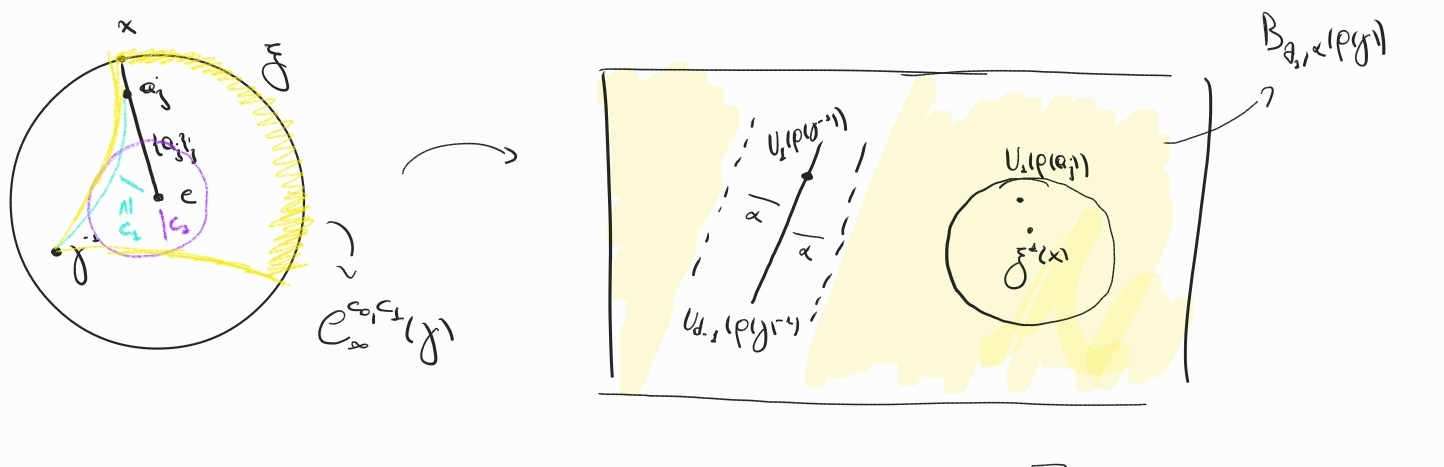
\includegraphics[width=0.8\textwidth]{cone.jpg}
\end{figure}
\chapter{Lower bound}
We denote with $\Pi$ the set of simple positive roots, and for $\Theta \subseteq \Pi$ we consider the Levi-Anosov subspace of $\mathfrak a$
\[
    \mathfrak a_\Theta = \bigcap_{\alpha \notin \Theta} \ker \alpha,
\]
which in particular admits $\{ \omega_{\alpha_i} : \alpha_i \in \Theta \}$ as a basis.
Finally, we shall consider the Busemann cocycle
\[
    b_\Theta : \PSL(d, \mathbb R) \times \mathcal F_\Theta \to \mathfrak a_\Theta
\]
which might as well be defined as
\[
    \omega_{\alpha_i}(b_\Theta(g, x)) =
    \log \frac{\| g v_1 \wedge \cdots g v_i \|}{ \| v_1 \wedge \cdots v_i \| }
    \text{ for all } \alpha_i \in \Theta
\]
for any basis $v_1, \ldots, v_i$ of $x^i \in \mathcal G_i(\mathbb R^d)$, where $\| \cdot \|$ denotes the norm on $\bigwedge^i \mathbb R^d$ induced by the euclidean inner product on $\mathbb R^d$, 
i.e.\ $ \langle v_1 \wedge \cdots \wedge v_k, w_1 \wedge \cdots \wedge w_k \rangle := \det(\langle v_i, w_j \rangle)$.
\begin{definition}
    For a discrete subgroup $\Gamma < \PSL(d, \mathbb R), \phi \in (\alpha_\Theta)^*$,
    a $(\Gamma, \phi)$-Patterson Sullivan measure on $\mathcal F_\Theta$ is a finite Radon measure $\mu$ such that for every $\gamma \in \Gamma$
    \[
        \frac{\d\gamma_* \mu}{\d\mu}(x) = e^{-\phi(b_\Theta(g^{-1},x))}, \text{ for all } x \in \mathcal F_\Theta(\mathbb R^d).
    \]
\end{definition}

\begin{lemma}\label{lem:busemann}
Let $\alpha > 0, \Theta \subseteq \Pi$.
There exists $K = K(\alpha) > 0$ such that for each $g \in \SL(d, \mathbb R), \sf{a_i} \in \Theta, y \in B_{\Theta, \alpha}(g)$
\[
    |\omega_i (a(g) - b(g, y))| \leq K.
\]
\end{lemma}\todo{How to prove this?}
Recalling that $\{ \omega_i \}_{\sf a_i \in \Theta} $ is a basis for $\mathfrak a_\Theta$, the above implies in particular that for each $\phi \in \mathfrak a_\Theta^*$ there exists $K = K(\alpha, \phi) > 0$ such that for all $g \in \SL(d, \mathbb R), y \in B_{\Theta, \alpha}(g)$
\[
    |\phi (a(g) - b(g, y))| \leq K.
\]
\section{Proof strategy}
Denoting with $d_\Gamma = \dim_H \xi_\rho^1(\partial \Gamma)$ the Hausdorff  dimension of the limit set, we shall outline how to obtain its lower bound by the Falconer dimension
\[
    d_\Gamma \geq h_\rho(F).
\]

First we recall that $F_s(a) = \max \{ \Psi_s^p(a) : p \in \llbracket 2, d \rrbracket\}$ and in particular $h_\rho(F) \leq h_\rho(\Psi^{d_\Gamma + 1})$.
Thus the lower bound will follow once we have shown that
$$d_\Gamma \geq h_\rho(\Psi^{d_\Gamma + 1}).$$

Noting that $(s+1) J_{d_\Gamma^u} \geq \Psi_{s+d_\Gamma}^{d_\Gamma + 1}$, the above bound will follow as soon as we have shown that
\begin{equation}\label{eq:JacobianBound}
    h_\rho(J_{d_\Gamma}) \geq 1.\tag{LB}
\end{equation}
To obtain \cref{eq:JacobianBound}, one uses the method of Patterson-Sullivan-Quint, which may be summed up in
\begin{align*}
    \text{There exists a } (\phi, \rho)\text{-Patterson-Sullivan measure on } \mathcal F_\Theta(\mathbb R^d) 
    \Rightarrow h_\rho(\phi) \geq 1,
\end{align*}
where $\phi \in \mathfrak a_\Theta$ and $ \Theta \subseteq \Pi$.
The property that we will need of our measure is that there exists a collection of open sets ${U_\gamma}_\gamma \in \Gamma$ such that
\begin{align*}\label{eq:GoodMeasure}
    \mu(U_\gamma) \sim e^{-J_{d_\Gamma}^u(a(\rho(\gamma)))} \text{ and } 
    M := \sup_{n \in \mathbb N}
    \max
    \left\{\sharp A : A \subseteq \Gamma_n,  \bigcap_{\gamma \in A}U_\gamma \neq \emptyset \right\} < \infty\tag{MP}
\end{align*}
where $\Gamma_n = \{ \gamma \in \Gamma : |\gamma| = n \} $.
The existence of a $(J_{d_\Gamma}^u, \rho)$-Patterson-Sullivan measure that satisfies the property (\ref{eq:GoodMeasure}) will be proved in \cref{sec:MeasureExistence}.
Assuming that for the time being, below we outline the Patterson-Sullivan-Quint method of obtaining \cref{eq:JacobianBound}.

Indeed, we first obtain the uniform in $n$ bound:
\begin{align*}
    \sum_{\gamma \in \Gamma_n}
    e^{-J_{d_\Gamma}^u(a(\rho(\gamma)))} \lesssim
    \sum_{\gamma \in \Gamma_n}
    \mu(\rho(U_\gamma)) \leq \frac{1}{M} \mu(\mathcal F_\Theta(\mathbb R^d)) < \infty
\end{align*}
along with the bound implied by the Anosov property of $\rho$:
\begin{align*}
J_{d_\Gamma}(a(\rho(\gamma))) \geq \mathsf a_{12} (a(\rho(\gamma))) \geq C|\gamma| - b
\end{align*}
to conclude that
\begin{align*}
\sum_{\gamma \in \Gamma} e^{-(s+1)J^u_{d_\Gamma}(a(\rho(\gamma)))} &=
\sum_{n\geq 0} \sum_{\gamma \in \Gamma_n} e^{-s J^u_{d_\Gamma}(a(\rho(\gamma)))}
    e^{J^u_{d_\Gamma}(a(\rho(\gamma)))} \lesssim
\sum_{n\geq 0} e^{-s(Cn - b)} < \infty
\end{align*}
which holds for any $s>0$, and thus \cref{eq:JacobianBound} holds.

\section{Existence of Patterson-Sullivan measure}\label{sec:MeasureExistence}
\begin{definition}
    Let $V \in \mathcal G_{p+1}{\mathbb R^d}$ and $l \in \mathbb P(V)$.
    Using the canonical identification $T_l \mathbb P(V) \simeq \hom (l, V/l)$, we define the density $|\Omega_{l, V}|$ on $\bigwedge^p T_l \mathbb P(V)$ by
    \[
        |\Omega_{l,V}|(\phi_1, \ldots, \phi_p) = 
        \frac{\| v \wedge \tilde \phi_1(v) \wedge \cdots \wedge \tilde \phi_p (v) \|}{\|v\|^{p+1}}
    \]
    for any $v \in l - \{ 0\}$, where $\tilde \phi_1, \ldots \tilde \phi_p \in \hom(l, V)$ are such that $\phi_i = \tilde \phi_i + \hom(l, l)$ and $\| \cdot \|$ denotes the norm on $\bigwedge^{p+1} R^d$ induced by the euclidean inner product.
\end{definition}

The following is \cite[Proposition 6.4]{pozzetti_anosov_2023}:
\begin{proposition}
Assume that $\xi^1_\rho(\partial \Gamma)$ is a Lipschitz submanifold of dimension $d_\Gamma$.
Then there exists a $(\rho(\Gamma), J_{d_\Gamma}^u)$-Patterson-Sullivan measure on $\mathcal F_{1,d_\Gamma + 1}$.
\end{proposition}
\begin{proof}
    By Rademacher's theorem, $\xi^1_\rho(\partial \Gamma)$ has a well-defined Lebesgue measure class, and Lebesgue-almost every $\xi^1_\rho(x) \in \xi^1_\rho(\partial \Gamma)$ admits a well-defined tangent space $T_{\xi^1_\rho(x)} \xi^1_\rho(\partial \Gamma)$.
    Considering such a $\xi^1_\rho(x)$ we let
    \[
        \pi : \hom(\xi^1_\rho(x), \mathbb R^d) \to \hom(\xi^1_\rho(x), \mathbb R^d/\xi^1_\rho(x)) \simeq T_{\xi^1_\rho(x)} \xi^1_\rho(\partial \Gamma),
    \]
    and
    \[
        x^{d_\Gamma + 1} = \pi^{-1} (T_{\xi^1_\rho(x)} \xi^1_\rho(\partial \Gamma)) \xi^1_\rho(x) \in 
        \mathcal G_{d_\Gamma + 1} (\mathbb R^d),
    \]
    for which one can show that
    \[
        T_{\xi^1_\rho(x)} \xi^1_\rho(\partial \Gamma) \simeq 
        \hom(\xi^1_\rho(x), \mathbb R^d / \xi^1_\rho(x)) \simeq
        \hom(\xi^1_\rho(x), x^{d_\Gamma + 1} / \xi^1_\rho(x)).
    \]
    In this notation, we shall define (Lebesgue-almost eeverywhere) the map
    \begin{align*}
        \zeta_\rho: \xi_\rho^1(\partial \Gamma) \to \mathcal F_{1, d_\Gamma + 1} (R^d), \quad 
        \zeta_\rho(\xi_\rho^1(x)) = (\xi_\rho^1(x), x^{d_\Gamma + 1}).
    \end{align*}

    We now define the non-negative density on $\xi_\rho^1(\partial \Gamma)$
    \[
        \mu_{\xi_\rho^1(x)} = |\Omega_{\zeta_\rho(\xi_\rho^1(x))}|
    \]
    which satisfies
    \[
        \frac{\d \gamma_*\mu}{\d\mu}(\xi) = \frac{\d (\rho(\gamma)^{-1})^*\mu}{\d\mu}(\xi) =
        e^{-J^u_{d_\Gamma + 1}(b_\Theta(\rho(\gamma)^{-1}, \zeta(x))))},
    \]
    where the term on the left-hand side involves measures, the term between the two equalities involves densities, and $\Theta = \{1, d_\Gamma + 1\}$.
    Indeed, for $\phi_1, \ldots, \phi_{d_\Gamma} \in T_{\xi_\rho^1(x)}\xi_\rho^1(\partial \Gamma)$:
    \begin{align*}
        &(\rho(\gamma)^*\mu)_{\xi_\rho^1(x)} (\phi_1, \ldots, \phi_{d_\Gamma})\\
        &=
        \mu_{\rho(\gamma)\xi_\rho^1(x)} (\rho(\gamma)\phi_1\rho(\gamma)^{-1}, \ldots, \rho(\gamma)\phi_{d_\Gamma} \rho(\gamma)^{-1}) =\\
        &=
        \frac{\|\rho(\gamma) \xi_\rho^1(x) \wedge \rho(\gamma) \phi_1(\xi_\rho^1(x)) \wedge \cdots \wedge \rho(\gamma) \phi_{d_\Gamma}(\xi_\rho^1(x))\|}{\| \rho(\gamma) \xi_\rho^1(x) \|^{d_\Gamma + 1}} =\\
        &=
        \frac{\|\rho(\gamma) \xi_\rho^1(x) \wedge \rho(\gamma) \phi_1(\xi_\rho^1(x)) \wedge \cdots \wedge \rho(\gamma) \phi_{d_\Gamma}(\xi_\rho^1(x))\|}
        {\|\xi_\rho^1(x) \wedge \phi_1(\xi_\rho^1(x)) \wedge \cdots \wedge \phi_{d_\Gamma}(\xi_\rho^1(x))\|} \cdot
        \frac{\|\xi_\rho^1(x) \wedge \phi_1(\xi_\rho^1(x)) \wedge \cdots \wedge \phi_{d_\Gamma}(\xi_\rho^1(x))\|}
        {\|\rho(\gamma) \xi_\rho^1(x)\|^{d_\Gamma+1}}\cdot
        \frac{\| \rho(\gamma)\xi_\rho^1(x)\|^{d_\Gamma+1}}{\|\xi_\rho^1(x)\|^{d_\Gamma+1}}
         =\\
         &=
         e^{\omega_{d_\Gamma}(b_\Theta(\rho(\gamma), \zeta_\rho(\xi_\rho^1(x))))} \cdot
         \mu_{\xi_\rho^1(x)}(\phi_1, \ldots, \phi_{d_\Gamma}) \cdot
         e^{-(p+1)\omega_1(b_\Theta(\rho(\gamma), \zeta_\rho(\xi_\rho^1(x))))} =\\
         &=
         e^{-J_{d_\Gamma}^u(b_\Theta(\rho(\gamma)^{-1}, \zeta(\xi_\rho^1(x)))} \mu_{\xi_\rho^1(x)}(\phi_1, \ldots, \phi_{d_\Gamma}).
    \end{align*}
    
    Finally, we let $\nu = {\zeta_\rho}_* \mu$, which is the wanted Patterson-Sullivan measure on $\mathcal F_{1, d_\Gamma + 1} (\mathbb R^d)$, since for $f \in C_c(\mathcal F_{1, d_\Gamma + 1} (\mathbb R^d))$:
    \begin{align*}
        \int_{\mathcal F_{1, d_\Gamma + 1} (\mathbb R^d)} f \d(\gamma_* {\zeta_\rho}_* \mu) &=
        \int_{\xi_\rho^1(\partial \Gamma)} f \circ \gamma \circ \zeta_\rho \d \mu =
        \int_{\xi_\rho^1(\partial \Gamma)} f \circ \zeta_\rho \circ \gamma \d \mu =\\
        &=
        \int_{\xi_\rho^1(\partial \Gamma)} f \circ \zeta_\rho(\xi) e^{-J_{d_\Gamma}^u(b_\Theta(\rho(\gamma)^{-1}, \zeta(\xi_\rho^1(x)))} \d \mu(\xi_\rho^1(x)) =\\
        &=
        \int_{\mathcal F_{1, d_\Gamma + 1} (\mathbb R^d)} 
        f(y) e^{-J_{d_\Gamma}^u(b_\Theta(\rho(\gamma)^{-1}, y)} \d ({\zeta_\rho}_*\mu)(y)
    \end{align*}
\end{proof}

Before giving the next definition, we recall that the annihilator annihilator of an element $y \in \mathcal F_F{i \Theta}(\mathbb R^d)$ is the set of partial flags that are not transverse to $y$, that is:
\[
    \mathrm{Ann}(y) = \left\{ x \in \mathcal F_{\Theta}(\mathbb R^d) : x^\theta \cap y^{d- \theta} \neq 0 \text{ for some } \theta \in \Theta \right\}.
\]
\begin{definition}
Let $\rho: \Gamma \to \SL(d,\mathbb R)$ be a linear representation, $\Theta \subseteq \Pi$ and $\mu$ a measure over $\mathcal F_\Theta(\mathbb R^d)$.
We say that $\rho$ is $\mu$-irreducible there is no element in $\mathcal F_{i \Theta}(\mathbb R^d)$, whose annihilator is of full measure, i.e.\ for all $y \in \mathcal F_{i \Theta}(\mathbb R^d)$:
\[
    \mu(\mathrm{Ann}(y)) < \mu(\mathcal F_{\Theta}(\mathbb R^d)).
\]
\end{definition}

\begin{example}
    If $\rho(\Gamma)$ is Zariski-dense in $\SL (d, \mathbb R)$, then $\rho$ is $\mu$-irreducible for any $\rho$-quasi-equivariant measure $\mu$, and in particular for any $(\rho(\Gamma), \phi)$-Patterson-Sullivan measure.
\end{example}

\begin{remark}
    The reason that we introduce the concept of $\mu$-irreducibility is that for any $\mu$-irreducible representation $\rho:\Gamma \to \SL{d,\mathbb R}$, there exist $\alpha, \kappa > 0$ such that $\mu(B_{\Theta, \alpha}(\rho(\gamma))) \geq k$ for all $\gamma \in \Gamma$.

    Indeed, if this were not the case, then there would exists a sequence $\alpha_n \searrow 0$ and $\gamma_n \in \Gamma$ such that
    \[
        \mu(B_{\theta, \alpha}(\rho(\gamma))) \leq \frac{1}{n}.
    \]
    Due to the compactness of $\mathcal F_{\Theta} (\mathbb R^d)$, up to considering a subsequence, we may assume that the reppeling flags or $\rho(\gamma_n)$ converge to some $\xi \in \mathcal F_{\Theta} (\mathbb R^d)$:
    \[
        (U_{d-i}(\rho(\gamma_n)^{-1}))_{\mathsf a_i \in \Theta} \to \xi
    \]
    
    In that case, the complements $B_{\Theta, \alpha_n}^c(\rho(\gamma_n))$ will converge to the annihilator of $\xi$, in the sense:
    \[
        \limsup_n B_{\Theta, \alpha_n}^c(\rho(\gamma_n)) \subseteq \mathrm{Ann}(\xi).
    \]
    Indeed, let $y\in \limsup_n  B_{\Theta, \alpha_n}^c(\rho(\gamma_n))$ and consider a subsequence $k_n$ such that $y\in B_{\Theta, \alpha_n}^c(\rho(\gamma_{k_n}))$.
    By the very definition of $B_{\Theta, \alpha_n}(\rho(\gamma_n))$, there exists some $p$ such that up to considering a subsequence of $k_n$,
    \[
        \angle (y^p, U_{d-p}(\rho(\gamma_n)^{-1})) \leq \alpha_n
    \]
    holds.
    Taking the limit as $n \to \infty$, we have that $y^p \cap \xi^{d-p} \neq 0$ and hence $y \in \mathrm{Ann(\xi)}$.

    Using a measure-theoretic arguement we conclude that $\mathrm{Ann}(\xi)$ is of full measure, which contradicts the $\mu$-irreducibility of $\rho$:
    \[
        \mu(\mathrm{Ann}(\xi)) \geq
        \mu (\limsup_n B_{\Theta, \alpha_n}^c(\rho(\gamma_{k_n})) ) \geq 
        \limsup_n \mu (B_{\Theta, \alpha_n}^c(\rho(\gamma_{k_n}))) =
        \mu(\mathcal F_\Theta (\mathbb R^d)).
    \]
\end{remark}

\begin{lemma}
    Let $\rho:\Gamma \to \SL(d, \mathbb R)$ be a representation and $\mu^\phi$ be a ($\rho(\Gamma), \phi$)-Patterson-Sullivan measure.
    If $\rho(\Gamma)$ is $\mu$-irreducible, then there exists some $\alpha_0 > 0$, such that for any $\alpha \in (0, \alpha_0)$, there's some $k = k(\alpha) > 0$ for which
    \[
        \frac{1}{k} e^{-\phi(a(\rho(\gamma)))} 
        \leq 
        \mu^\phi(\rho(\gamma) B_{\Theta, \alpha}(\rho(\gamma))) 
        \leq
        k e^{-\phi(a(\rho(\gamma)))} 
    \]
    for all $\gamma \in \Gamma$. 
\end{lemma}
\begin{proof}
    Let $\alpha_0, k > 0$ be as in the remark preceeding the statement of the lemma.
    As noted in \cref{lem:busemann}, there exists some $K = K(\alpha_0, \phi) > 0$ such that for any $\alpha \in (0, \alpha_0)$ and $y \in B_{\Theta, \alpha}(\rho(\gamma))$:
    \[
        |\phi(a(\rho(\gamma)) - b(\rho(\gamma), y))| \leq K,
    \]
    from which we obtain the upper bound
    \begin{align*}
        \mu^\phi(\rho(\gamma) B_{\Theta, \alpha}(\rho(\gamma))) &=
        (\rho(\gamma^{-1})_*\mu^\phi)(B_{\Theta, \alpha}(\rho(\gamma))) =
        \int_{\mathcal F_\Theta(\mathbb R^d)} e^{-\phi(b(\rho(\gamma), y))} d\mu^\phi(y)\leq\\
        &\leq
        e^{-K} \mu^\phi(\mathcal F_\Theta (\mathbb R^d)) e^{-\phi(a(\rho(\gamma)))}.
    \end{align*}
    
    Similarly we obtain the lower bound
\end{proof}

*Appendix
\appendix
\chapter{Tangent space to the Grassmanian}
Let $V$ be a $d$-dimensional real vector space. 
We denote with $\mathcal G_{k}(V)$ the Grassmanian of $k$-dimensional subspaces of $V$.
Our first objective is to find a convenient way to express its tangent space.
\begin{proposition}
We have the following canonical identification:
\begin{align*}
    \hom(W, V/W) &\simeq T_W \mathcal G_{k}(V)\\
    \phi &\mapsto \frac{\d}{\d t} \Big|_{t=0} \Gamma(t \phi)
\end{align*}
where $\Gamma(\phi) = (Id+\phi)(W)$ is the graph of $\phi$.
\end{proposition}
\begin{proof}
    We will consider the map
    \begin{align*}
        F: \mathrm{Injhom}(W, V) \to \mathcal G_{k}(V), \quad \phi \mapsto \phi(W).
    \end{align*}
    whose derivative is given by:
    \begin{align*}
        d_I F (\phi) = F \left(\frac{\d}{\d t} \Big|_{t=0} (I + t\phi)\right)
        = \frac{\d}{\d t} \Big|_{t=0}  \left( I + t\phi (W) \right)
        = \frac{\d}{\d t} \Big|_{t=0}  \Gamma(t \phi).
    \end{align*}
    The result will follow as soon as we have shown that $d_I F$ is surjective and that $\ker d_I F = \hom(W, W)$.
    
    To show that it is surjective, we consider a $(d-k)$-dimensional subspace $W' \in \mathcal G_{d-k}(V) $ that is complementary to $W$, i.e.\ $V = W \oplus W'$.
    Denoting with $U_{W'} = \{ Z \in \mathcal G_k (V): Z \cap W' = 0 \}$, we recall the corresponding chart:
    \begin{align*}
        \Psi: \hom(W, W') &\to U_{W'}\\
        \phi &\mapsto \Gamma(\phi).
    \end{align*}
    Surjectivity of $d_I F$ now follows by the fact that
    \[
        d_I F(\phi) = \frac{\d}{\d t} \Big|_{t=0} \Gamma(t \phi) = d_0 \Psi(\phi).
    \]

    To show that $\ker d_I F = \hom(W, W)$, we first note that clearly $\ker \d_I F \supseteq \hom(W, W)$.
    Equality then follows by the fact that $\dim \hom(W, W) = \dim \ker \d_I F$, which is a direct consequence of the surjectivity.
\end{proof}

Note that another way to prove the above identification throught the fact that the Grassmanian is a homogeneous space of $\GL(d, \mathbb R)$, giving us the diffeomorphism
\begin{align*}
    \GL(V) / \mathrm{St}_{GL(V)} W &\to \mathcal G_k(V)\\
    [g] &\mapsto gW,
\end{align*}
where $\mathrm{St}_{GL(V)} W = \{ g \in \GL(V) : gW = W \}$ is the stabilizer of $W$.
Thus an expression for the tangent space at $W$ may be obtained by differentiating the map above at the identity coset:
\begin{align*}
    \hom(W, V/W) \simeq \hom(V, V) / \hom(W, W) &\simeq T_W \mathcal G_k(V).
\end{align*}
In particular the above gives us a direct proof that the kernel of the map constructed in the previous proof is indeed $\hom(W, W)$.
\end{document}